\section{Internship accomplishments}
\label{sec:accomplish}

This section describes the main tasks achieved during the traineeship, along with the reason why they were needed, the way they have been implemented and the knowledge that they brought.

\subsection{Building of UI components}
\label{ssec:ui_components}

As mentioned in {\sc subsection}~\ref{ssec:frameworks}, ReactJS is based on encapsulated components, most of them appearing several times on the website. They can be very basic (e.g. buttons) or more elaborate (e.g. modals). For this reason, it is a good idea to create a library of generic components, that can be reused as many times as required. This saves a lot of development time, and also assures a certain homogeneity between the different pages of the application.

Several developers, including myself, built this library in a folder named \guillemotleft{} ui \guillemotright{}. One of the components that I have created is the \guillemotleft{} DatePicker \guillemotright{}. Since this is a rather complex component, a good reflex is to first take a look at existing ReactJS plugins. They are usually hosted on Github, with a demonstration link of how they behave and a quick download option via npm.

I found a few possible date pickers, so a selection had to be made, based on several criteria. One of them is the latest update of the repository: if it is quite recent, it means that the owner can quickly help in case there is any problem with the plugin. Also, if the repository has a lot of stars, it means that lots of people using it are satisfied. Another good sign is a low number of open issues in the repository. In the end, the choice was a plugin called \guillemotleft{} react-datepicker \guillemotright{}~\footnote{https://github.com/Hacker0x01/react-datepicker}.

Then, to start the implementation, a \guillemotleft{} DatePicker \guillemotright{} folder was added to the library of components. In this new folder, I created a file named \textit{DatePicker.js} which contains the code of the component. At the top of this file are a few \guillemotleft{} import \guillemotright{} statements, as seen on {\sc figure}~\ref{fig:imports}: ReactJS, the previously downloaded plugin, and also \textit{DatePicker.scss}.

\begin{figure}[H]
    \centering
    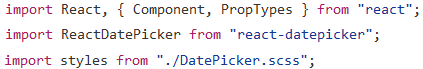
\includegraphics[scale=0.9]{figure/imports.png}
    \caption{The needed importations for the DatePicker UI component.}
    \label{fig:imports}
\end{figure}

This last imported file contains the local CSS styles for the date picker, that will not be used anywhere else in the application. This system makes sure that if changes are made in the CSS for one component, they will not affect other UI elements. However, Konnektid uses some global CSS values (fonts, colors, etc) that are defined in SCSS files at the root of the \guillemotleft{} ui \guillemotright{} folder. Those are meant to be reused in every component, to make the website more harmonious. So I used them to customize react-datepicker, and the final result is presented on {\sc figure}~\ref{fig:datePicker}.

\begin{figure}[H]
    \centering
    
\includegraphics[scale=0.6]{figure/datePicker.png}
    \caption{The final DatePicker presentational component.}
    \label{fig:datePicker}
\end{figure}

This assignment was an efficient way to learn JavaScript and some good ReactJS practices. Moreover, it was a great introduction to the ReactJS community and all the support that it brings, especially with the numerous plugins that are shared.

\subsection{Implementation of new pages}
\label{ssec:new_pages}

It has been explained in {\sc subsection}~\ref{ssec:concept} that Konnektid's main goal for the year is to test and validate their business model, which relies on
professional teachers. This requires the implementation of several new pages and functionalities, and some have been built during the internship. Among them, only
two will be described here: first the course page, then the teachers landing page.

\subsubsection{The course page}
\label{sssec:coursePage}

The course page refers to the page used for teachers to create, edit and publish a course. It had to be built from scratch, for both desktop and mobile, based on designs
made by Konnektid's former designer. It is now released and used by professional teachers, and an example is visible on {\sc figure}~\ref{fig:coursePage}.

\begin{figure}[H]
    \centering
    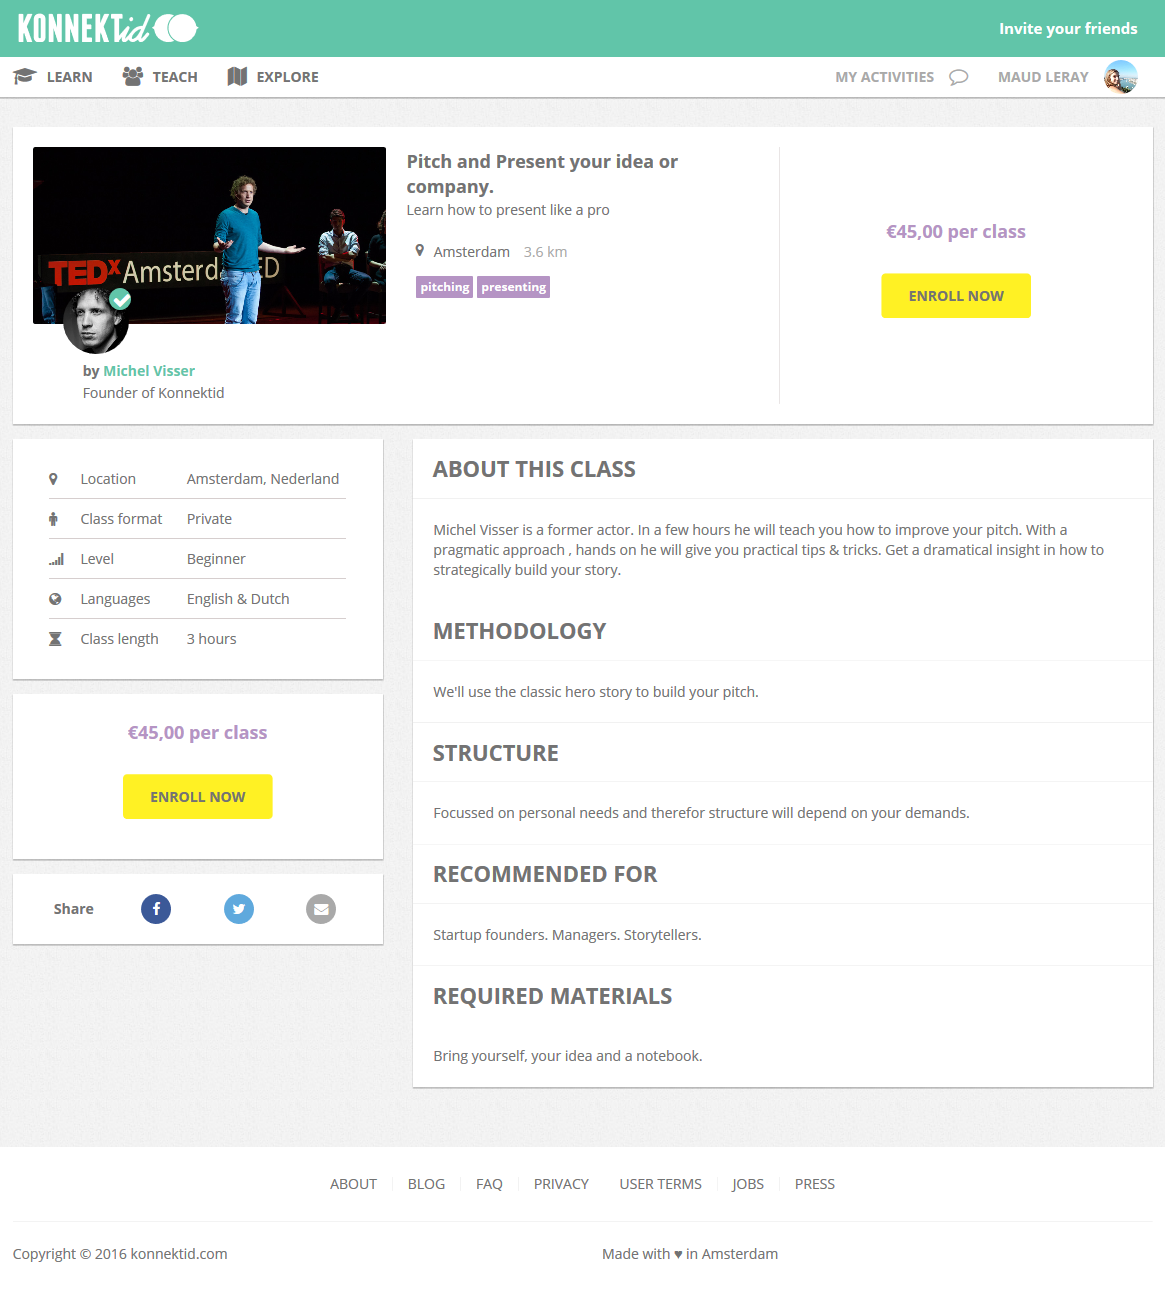
\includegraphics[scale=0.2]{figure/coursePage.png}
    \caption{An example of course published on the website (desktop version).}
    \label{fig:coursePage}
\end{figure}

We can see that the page features two main elements:

\textbf{The top section} which contains all the main information about the course (picture, title, price\ldots) and the teacher (avatar, name, short introduction).
The teacher name is a direct link to his or her profile. On the right, this section also provides a button \guillemotleft{} Enroll now \guillemotright{} for the students
to book the course.

\textbf{The bottom section} which is divided in two parts. The right part takes most space on the page and gives an in-depth description of the course
(methodology, requirements\ldots). The left part, which is thinner, shows practical information about the course (format, length\ldots) and another
\guillemotleft{} Enroll now \guillemotright{} button with a reminder of the price. Below this are all the sharing functionalities: Facebook, Twitter,
email, and even WhatsApp on mobile.

This was the very first whole JavaScript page I implemented. It made me realize the value of the components library mentioned in {\sc subsection}~\ref{ssec:ui_components}.
Indeed, it is really convenient to have all these built-in UI components to reuse, and it makes building interfaces much faster. The biggest challenge here was to divide
the page in smaller sub-components, each of them in their own folder with local CSS styles. For instance, the biggest bottom part is a component called
\guillemotleft{} CourseDescriptionCard \guillemotright{}. Since it contains several sections that are very similar in presentation and only differ by their title and content,
it made sense to create a reusable \guillemotleft{} CourseDescriptionItem \guillemotright{} to render them with title and content passed down as props. This is a recommanded
practice, as it respects the single responsibility principle previously mentioned in {\sc subsection}~\ref{ssec:frameworks} and avoids duplicated code.
These are two of the many techniques for writing maintainable code~\cite{maintainable}, i.e. code that is easy to read, to modify and to extend.

After the static course page has been built and reviewed, my tutor asked me to add inline editing for the teachers to edit their courses.
This means that all elements can be edited in-place, in the context where they will be published, which facilitates picturing the final result.
In order to implement this, I used a rich text editor framework for ReactJS called \textit{DraftJS}.

DraftJS enables the creation of rich content, such as bold or italic text and lists of items. These features are available for the teachers when editing the
CourseDescriptionCard. But they can also be blocked, for instance when editing the title of the course which needs to be a simple line.

\begin{figure}[H]
    \centering
    
\includegraphics[scale=0.2]{figure/courseEditIntro.png}
    \caption{The top section of the course page when being edited.}
    \label{fig:courseEditIntro}
\end{figure}

\subsubsection{The teachers landing page}
\label{sssec:teachersPage}

\begin{itemize}
    \item Teachers landing page => interesting because did everything from wireframe/design to implementation
\end{itemize}

\subsection{Creation of flows}
\label{ssec:flows}

\textbf{Not sure if necessary, as wireframes are already mentioned in the previous subsection?}

Matchmaking flow

\subsection{New navigation}
\label{ssec:new_nav}

\begin{itemize}
    \item Responsible of the project
    \item Added feature flag, new navigation in old pages for both mobile and desktop, only in desktop for new pages
\end{itemize}

\subsection{Analytics}
\label{ssec:analytics}

\begin{itemize}
    \item Updated analytics in old pages (for instances for inviting friends)
    \item Added analytics to new pages (explain new analytics and maybe necessary refactoring for enroll modal)
\end{itemize}

In addition to the technical learnings, this internship has been a great occasion to dive into the startup life and to discover the process of company building. This requires a solid project management system, and the one used at Konnektid is explained in {\sc section}~\ref{sec:management}.